\chapter{自旋、同位旋、色与胶子自相互作用}

\section{通过与电动力学的类比理解量子色动力学}

量子色动力学是一个过于庞大的课题，无法在一次讲座中完整展开。这里的目标是给出基本的直观图像，而不是更深入的数学。

量子电动力学是关于电子和光子的理论。它也是关于库仑力的量子理论。如果把原子核视为一个固定的电场源，而不追问其运动或内部结构，那么QED就是关于原子的理论。

量子色动力学对夸克和胶子起着类似的作用。它描述这些粒子本身、它们之间的力，以及它们所形成的复合对象。这些复合对象称为\emph{强子}。质子和中子是重子：它们携带净夸克数，等价地说，携带非零的重子数。介子是夸克--反夸克组合。重子和介子也都包含胶子。

胶子不带电，但它们提供了束缚夸克的场。在这一方面，胶子场所起的作用类似于束缚原子的电磁场。

在引入色和胶子之前，回到自旋的数学是有益的。同样的数学几乎直接再次出现为\emph{同位旋}，而一个相关的模式在色理论中再次出现。群论是这些构造的基础，但所需的思想可以通过角动量来展开。

\section{角动量多重态}

角动量的各分量满足
\begin{equation}
[L_x,L_y]=i\hbar L_z,
\end{equation}
以及循环相伴关系
\begin{equation}
[L_y,L_z]=i\hbar L_x,
\qquad
[L_z,L_x]=i\hbar L_y.
\end{equation}
这三个分量不对易，因此不能同时测量。于是，一种描述会选定一个轴，通常取\(z\)轴，并用沿该轴的角动量分量来标记态。

这一选择并不破坏自然界中的旋转对称性。它只是在描述中破坏了对称性，即为记账选定了一个方向。

\(z\)分量的允许值是量子化的，并且相差一个\(\hbar\)单位。在列出这些值时取\(\hbar=1\)，一个自旋为\(\ell\)的多重态包含
\begin{equation}
m=\ell,\ell-1,\ldots,-\ell.
\end{equation}
因此，独立态的数目为
\begin{equation}
2\ell+1.
\end{equation}

前几个多重态值得明确写出：
\begin{align}
\ell=0:&\qquad m=0,\\
\ell=\frac12:&\qquad m=\frac12,-\frac12,\\
\ell=1:&\qquad m=1,0,-1,\\
\ell=\frac32:&\qquad
m=\frac32,\frac12,-\frac12,-\frac32,\\
\ell=2:&\qquad m=2,1,0,-1,-2.
\end{align}

就目前的目的而言，半整数自旋属于费米子，整数自旋属于玻色子。电子是自旋为\(\tfrac12\)的粒子。自旋为零的粒子完全没有角动量。光子自旋为一，自旋为一的态也出现在原子和原子核中。原子和原子核同样可以具有自旋\(\tfrac32\)，而同样的计数会继续到更高的自旋。

记号必须区分总自旋与其分量。数\(\ell\)标记多重态，同时也是\(z\)分量的最大可能值。数\(m\)标记该多重态中的某个特定态。因此，一个自旋为一的对象有三个态，而一个自旋为\(\tfrac12\)的对象有两个态。

\section{两个自旋半粒子的组合}

考虑两个自旋为\(\tfrac12\)的粒子，并忽略它们的轨道角动量。它们的自旋乘积空间包含四个基态：
\begin{equation}
|\uparrow\uparrow\rangle,\qquad
|\uparrow\downarrow\rangle,\qquad
|\downarrow\uparrow\rangle,\qquad
|\downarrow\downarrow\rangle.
\end{equation}
相应的\(z\)分量为
\begin{align}
|\uparrow\uparrow\rangle &: m=+1,\\
|\uparrow\downarrow\rangle &: m=0,\\
|\downarrow\uparrow\rangle &: m=0,\\
|\downarrow\downarrow\rangle &: m=-1.
\end{align}

两个自旋都向上的态证明必然出现一个自旋为一的多重态：最大的\(z\)分量为\(+1\)。一个自旋为一的多重态只有三个态，
\begin{equation}
m=+1,\quad 0,\quad -1.
\end{equation}
但乘积空间包含四个态，其中包括两个\(m=0\)的独立态。它们不可能都属于同一个自旋为一的多重态。多出的态不可能是自旋二，因为一个自旋二的多重态需要五个态。因此，这四个乘积态必须分为三个自旋为一的态和一个自旋为零的态。

两个\(m=0\)基态的哪种组合属于自旋为一的多重态？交换这两个粒子。对齐的态不变：
\begin{equation}
|\uparrow\uparrow\rangle\longrightarrow|\uparrow\uparrow\rangle,
\qquad
|\downarrow\downarrow\rangle\longrightarrow|\downarrow\downarrow\rangle.
\end{equation}
相比之下，混合乘积态被交换：
\begin{equation}
|\uparrow\downarrow\rangle
\longleftrightarrow
|\downarrow\uparrow\rangle.
\end{equation}
它们的和在交换下是对称的：
\begin{equation}
|\uparrow\downarrow\rangle+|\downarrow\uparrow\rangle.
\end{equation}
归一化给出一个因子\(1/\sqrt2\)：
\begin{equation}
|1,0\rangle
=
\frac{|\uparrow\downarrow\rangle
      +|\downarrow\uparrow\rangle}{\sqrt2}.
\end{equation}

\begin{figure}[h]
\centering
\includegraphics[width=0.78\textwidth]{lecture_02_figure_02.png}
\caption{形成自旋一三重态中\(m=0\)成员的对称混合自旋组合。}
\lectureframe{00:15:08}
\end{figure}

与两个对齐的态一起，这给出自旋一三重态：
\begin{align}
|1,+1\rangle &=|\uparrow\uparrow\rangle,\\
|1,0\rangle &=
\frac{|\uparrow\downarrow\rangle
      +|\downarrow\uparrow\rangle}{\sqrt2},\\
|1,-1\rangle &=|\downarrow\downarrow\rangle.
\end{align}
剩余的相互正交的组合带有一个负号：
\begin{equation}
|0,0\rangle
=
\frac{|\uparrow\downarrow\rangle
      -|\downarrow\uparrow\rangle}{\sqrt2}.
\end{equation}
它在交换下是反对称的，并形成单态的自旋为零多重态。因此
\begin{equation}
\frac12\otimes\frac12=1\oplus0.
\end{equation}

对称的混合自旋态具有\(m=0\)，但它\emph{并不}具有零总角动量。它属于自旋三重态。旋转坐标轴会将它和\(m=\pm1\)态混合。只有反对称组合才具有\(\ell=0\)。

就角动量而言，单态就像空无一物的空间。它可能携带能量、电荷或其他量子数，但它不携带角动量。

这一区别可以通过一个思想实验来检验。忽略除角动量守恒之外的所有守恒定律，并问：哪一种两粒子自旋态可以简单地消失？两个对齐态都不能消失，因为它们各自属于一个自旋为一的多重态。对称的\(m=0\)态也不能消失。尽管它的\(z\)分量消失，它的总自旋仍然是一，相对于其他轴具有非平凡分量。只有反对称单态可以在不违反角动量守恒的情况下消失。

\begin{classroomqa}
\audiencequestion{沿\(z\)轴测量对称的混合自旋态，会得到\(+1\)还是\(-1\)？\lecturetimestamp{00:19:28}}
\lecturerresponse{不会。沿\(z\)轴它给出零。然而该态的总自旋为一，因此沿另一轴测量可以给出\(+1\)或\(-1\)。}
\end{classroomqa}

\section{三个自旋半粒子}

现在组合三个自旋为\(\tfrac12\)的粒子。共有
\begin{equation}
2\times2\times2=8
\end{equation}
个乘积态。如果三个自旋都朝上，总\(z\)分量为\(+\tfrac32\)。因此必定存在一个自旋为\(\tfrac32\)的多重态。它包含
\begin{equation}
2\left(\frac32\right)+1=4
\end{equation}
个态。

还剩下四个态。它们不能构成第二个自旋为\(\tfrac32\)的多重态，因为具有\(m=\pm\tfrac32\)的态已经被用掉了。剩余态的最大分量只有\(+\tfrac12\)和\(-\tfrac12\)。三个半整数自旋也不能构成总自旋为零。剩余态必定构成自旋为\(\tfrac12\)的多重态。

一个自旋为\(\tfrac12\)的多重态包含两个态。既然还剩下四个态，就有两个不同的自旋为\(\tfrac12\)的多重态：
\begin{equation}
\frac12\otimes\frac12\otimes\frac12
=
\frac32\oplus\frac12\oplus\frac12.
\end{equation}
当被称为自旋向上和自旋向下的两个态被替换为被称为上夸克和下夸克的两个夸克味时，这一模式将再次出现。

\section{作为内部自旋的同位旋}

同位旋，或称同位素自旋，是普通自旋的内部类似物。普通自旋与物理空间的旋转相联系。同位旋则不然。它涉及一个内部数学空间中的变换，该空间的两个基本态将被等同于
\begin{equation}
u,\qquad d.
\end{equation}
这里的\emph{上}和\emph{下}仅仅是味标签。在普通空间中没有任何东西指向上方或下方。

\editorialnote{在内部自旋空间的定义与随后的强子质量尺度论证之间的一段简短过渡无法可靠地恢复。不从中推断任何额外的物理主张。}

为什么\(u\)和\(d\)适合这一类比？强子物理的天然能量尺度是几百MeV。一个典型轻介子的质量为几百MeV，将三个夸克束缚成核子所涉及的能量同样处于这一尺度。相比之下，普通原子核的结合能只有几MeV。因此，将质子和中子束缚在原子核内部的力，是在比将夸克束缚在强子内部的动力学小得多的能量尺度上被考虑的。

在六种夸克味中，\(u\)和\(d\)相对于强子尺度是轻的。重夸克产生需要更多能量，而含有重夸克的强子可以衰变为较轻的强子。因此最稳定的轻强子由上夸克和下夸克构成。

下夸克比上夸克重，在此处使用的估计中大约重两倍，但两者的质量相对于几百MeV都很小。在一级近似下，它们在强子尺度上都可以被当作几乎无质量。更重要的是，它们可以被当作质量几乎相等。

这种近似相等导致了一种对称性。如果交换上夸克和下夸克，强相互作用物理变化很小。质子，
\begin{equation}
p\sim uud,
\end{equation}
和中子，
\begin{equation}
n\sim udd,
\end{equation}
提供了最简单的例子：它们通过交换\(u\)和\(d\)而不同，并且它们的质量非常接近。

因此，交换
\begin{equation}
u\longleftrightarrow d
\end{equation}
在数学上被当作
\begin{equation}
|\uparrow\rangle\longleftrightarrow|\downarrow\rangle.
\end{equation}
来处理。对于普通自旋，该变换对应于空间中一个轴的旋转。对于同位旋，它是内部空间中的旋转。尽管物理含义不同，数学是类似的。

\begin{figure}[h]
\centering
\includegraphics[width=0.80\textwidth]{lecture_02_figure_03.png}
\caption{两个自旋\(\tfrac12\)态的三重态与单态分解，即相应同位旋构造的模型。}
\lectureframe{00:27:42}
\end{figure}

前缀\emph{iso}来自\emph{isotope}。在较早的核描述中，质子和中子被视为同一个内部二重态的两个成员。在原子核中交换质子和中子会把一种同位素变成另一种同位素。夸克模型后来把这种质子-中子交换追溯到\(u\)与\(d\)之间的底层交换。

\begin{classroomqa}
\audiencequestion{同位旋是否先于夸克模型出现？\lecturetimestamp{00:30:19}}
\lecturerresponse{是的。同位旋在夸克之前就被引入，历史上与海森堡相关。夸克模型后来为它提供了\(u\)和\(d\)味的解释。}
\end{classroomqa}

同位旋并不是自然界的一种精确对称性。上夸克和下夸克的质量并不完全相等，而且它们具有不同的电荷：
\begin{equation}
Q(u)=+\frac23,
\qquad
Q(d)=-\frac13.
\end{equation}
即使它们的质量相等，电磁相互作用仍然会把它们区分开来。

对于小的强子和核系统，电磁效应相比强相互作用是弱的。在大原子核中，电排斥可能变得重要；对于质子、中子或诸如氦这样的小原子核，它相对于强相互作用尺度是较小的修正。因此，同位旋近似由两步组成：

\begin{enumerate}
\item 忽略\(u\)--\(d\)质量差；
\item 关闭它们的电磁区分，只保留强相互作用。
\end{enumerate}

在该近似中，\(u\)与\(d\)之间的变换成为一种在数学上类似于普通自旋对称性的对称性。

\section{核子同位旋二重态}

单个夸克不能被孤立出来并作为自由实验室客体加以考察。最简单的已观测重子包含三个夸克。因此，三自旋计数论证有一个直接的同位旋类比：三个同位旋为\(\tfrac12\)的夸克可以形成总同位旋\(\tfrac32\)或\(\tfrac12\)。

从总同位旋\(\tfrac12\)开始。这样的多重态有
\begin{equation}
2\left(\frac12\right)+1=2
\end{equation}
个态。它们就是质子和中子：
\begin{equation}
p\sim uud,
\qquad
n\sim udd.
\end{equation}
它们的电荷为
\begin{align}
Q(p)
&=\frac23+\frac23-\frac13
=+1,\\
Q(n)
&=\frac23-\frac13-\frac13
=0.
\end{align}
交换\(u\)与\(d\)会交换质子和中子。它们形成一个同位旋为\(\tfrac12\)的二重态。

为了讨论交换对称性，暂时用\(1,2,3\)标记三个夸克槽位。这些标记不应被误认为固定的夸克位置；夸克在运动。一个示意性的质子因子是
\begin{equation}
d_1\bigl(u_2u_3-u_3u_2\bigr).
\end{equation}

\begin{figure}[h]
\centering
\includegraphics[width=0.58\textwidth]{lecture_02_figure_04.png}
\caption{示意性质子态中反对称化的两个\(u\)夸克因子。}
\lectureframe{00:35:43}
\end{figure}

该表达式的目的是强调费米子交换反对称性。它并不是完整的质子波函数。完整态必须结合味、普通自旋、空间依赖性以及---很快将变得至关重要的---色。

\editorialnote{下标是临时的槽位或单粒子标记。两个相同的\(u\)味态并不构成通常的反对称同位旋单态，因此所显示的因子本身并不支持同位旋为零的结论。它仅作为局部的槽位反对称化步骤而保留；质子的总同位旋来自其完整的三夸克态。}

与先前自旋构造的有限比较在于：量子态在标记交换下可以对称地或反对称地组合。仅凭这一比较并不能确定所显示的\(uu\)因子所携带的同位旋。

质子既有普通自旋\(\tfrac12\)，又有同位旋\(\tfrac12\)。中子也是如此。这些是不同的量子数：普通自旋涉及物理转动，而同位旋涉及\(u\)--\(d\)内部对称性。

\section{Delta四重态}

三个轻夸克也可以形成总同位旋\(\tfrac32\)。由此得到的四态多重态就是Delta四重态：
\begin{equation}
\begin{aligned}
\Delta^{++}&\sim uuu,
&
\Delta^{+}&\sim uud,
\\
\Delta^{0}&\sim udd,
&
\Delta^{-}&\sim ddd.
\end{aligned}
\end{equation}
Delta态既有普通自旋\(\tfrac32\)，也有同位旋\(\tfrac32\)。在具有最大分量的态中，三个普通自旋对齐，三个同位旋也对齐。

诸如\(uud\)这样的组成本身并不能确定该态是质子还是\(\Delta^+\)。相同的味内容可以组合成不同的总自旋态和总同位旋态。

\begin{classroomqa}
\audiencequestion{是什么把Delta四重态中的\(uud\)成员与质子区分开来？\lecturetimestamp{00:41:08}}
\lecturerresponse{它们的普通自旋不同。质子具有自旋\(\tfrac12\)，而Delta态具有自旋\(\tfrac32\)。夸克也被组合成不同的总同位旋态。}
\end{classroomqa}

\begin{classroomqa}
\audiencequestion{Delta 四重态的中间成员是同位旋-\(\tfrac12\)态吗？\lecturetimestamp{00:41:52}}
\lecturerresponse{不是。它们的同位旋分量是 \(+\tfrac12\) 和 \(-\tfrac12\)，但它们的总同位旋是 \(\tfrac32\)。一个总同位旋为 \(\tfrac32\) 的多重态必然包含四个分量态。}
\end{classroomqa}

这四个同位旋分量对应于
\begin{equation}
I_3=\frac32,\frac12,-\frac12,-\frac32.
\end{equation}
它们的电荷为
\begin{align}
Q(\Delta^{++})&=+2,\\
Q(\Delta^{+})&=+1,\\
Q(\Delta^{0})&=0,\\
Q(\Delta^{-})&=-1.
\end{align}
中间两个电荷恰好等于质子和中子的电荷，但这些态仍然不同，因为它们的自旋和同位旋耦合方式不同。

近似同位旋对称性使四个 Delta 的质量几乎相等。微小的 \(u\)--\(d\) 质量差只在四重态内产生很小的分裂。Delta 的共同质量尺度大致为
\begin{equation}
m_\Delta\sim1200\,\mathrm{MeV},
\end{equation}
而质子和中子则接近
\begin{equation}
m_N\sim940\,\mathrm{MeV}.
\end{equation}

\subsection{\texorpdfstring{\(\Delta^{++}\)}{Delta++}的衰变}

Delta 态足够重，可以衰变为一个核子和一个 {\proseunicodefont π} 介子。考虑
\begin{equation}
\Delta^{++}\sim uuu.
\end{equation}
当组分分离时，可以产生一个夸克--反夸克对。若试图插入 \(u\bar u\)，末态中会留下一个三-\(u\)重子，并且不能利用可用能量提供一个更轻的允许道。相反，产生一个 \(d\bar d\) 对则允许组分重新组合为
\begin{equation}
uuu+d\bar d
\longrightarrow
uud+u\bar d.
\end{equation}
两个末态复合粒子是
\begin{equation}
uud=p,
\qquad
u\bar d=\pi^+,
\end{equation}
因此
\begin{equation}
\Delta^{++}\longrightarrow p+\pi^+.
\end{equation}

\begin{figure}[h]
\centering
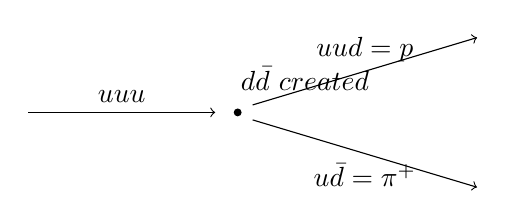
\begin{tikzpicture}[scale=0.95]
\draw[->] (-3,0) -- (-0.5,0) node[midway,above] {$uuu$};
\fill (-0.2,0) circle (1.5pt);
\draw[->] (0,0.1) -- (3,1.0) node[midway,above] {$uud=p$};
\draw[->] (0,-0.1) -- (3,-1.0) node[midway,below] {$u\bar d=\pi^+$};
\node at (0.7,0.45) {$d\bar d\ \text{created}$};
\end{tikzpicture}
\caption{衰变 \(\Delta^{++}\rightarrow p+\pi^+\) 中的组分重新组合。}
\end{figure}

电荷守恒是显然的：
\begin{equation}
Q(p)+Q(\pi^+)=1+1=2=Q(\Delta^{++}).
\end{equation}
粗略的质量平衡也允许该衰变：
\begin{equation}
1200\,\mathrm{MeV}
>
940\,\mathrm{MeV}+140\,\mathrm{MeV}.
\end{equation}
剩余能量足以在末态中提供动能。

所有四个 Delta 态都可以衰变为一个质子或中子以及一个 {\proseunicodefont π} 介子。它们的寿命极短。一个数量级估计是光穿过一个质子所需的时间：
\begin{equation}
\tau_\Delta
\sim
\frac{10^{-13}\,\mathrm{cm}}
     {10^{10}\,\mathrm{cm/s}}
\sim10^{-23}\,\mathrm{s}.
\end{equation}
尽管如此，它们的寿命仍长到足以被识别为粒子碰撞中产生的不同客体。

\begin{classroomqa}
\audiencequestion{在这种组分记账中，\(u\) 和 \(d\) 符号的书写顺序重要吗？\lecturetimestamp{00:48:49}}
\lecturerresponse{就当前目的而言不重要。重要的信息是味内容以及完整量子态的合成方式。}
\end{classroomqa}

\section{泡利难题与颜色的必要性}

\(\Delta^{++}\) 暴露出一个矛盾。它由三个上夸克组成。在自旋-\(\tfrac32\)态中，它们的普通自旋可以全部指向同一方向。它们的同位旋也相同，因为它们全都是 \(u\)。如果自旋、味和最低能量空间态就是全部描述，那么这三个夸克将是占据同一状态的相同费米子。泡利不相容原理禁止这一点。

\begin{classroomqa}
\audiencequestion{如果重复的上夸克似乎占据同一状态，它们怎么可能是费米子？\lecturetimestamp{00:48:58}}
\lecturerresponse{它们不可能在每个量子数上都相同。\(\Delta^{++}\) 表明，夸克需要除普通自旋、味和空间态之外的额外标签。这个额外标签就是颜色。}
\end{classroomqa}

这个新标签有三个可能取值：
\begin{equation}
r,\qquad g,\qquad b,
\end{equation}
称为红、绿、蓝。这些词与可见颜色毫无关系。它们只是三个内部态的任意名称。也可以使用其他名称；重要的是存在三种不同的可能性。

给定夸克味的红、绿、蓝版本具有相同的质量和相同的普通可观测性质。尽管如此，它们是不同的量子态。因此一个 \(\Delta^{++}\) 可以包含一个红色 \(u\)、一个绿色 \(u\) 和一个蓝色 \(u\)，所以这三个费米子并不占据同一个完整状态。

六种味是
\begin{equation}
u,\ d,\ c,\ s,\ t,\ b.
\end{equation}
这个顺序不是按质量排列的。上夸克最轻，下夸克次之。粲夸克比奇异夸克重得多，而顶夸克比底夸克重得极多。每一种味都有三种颜色。因此一个夸克至少携带两个不同的内部标签：
\begin{equation}
\text{flavor}\quad\text{and}\quad\text{color}.
\end{equation}

这三个夸克能否改用位置或动量来区分？Delta 难题涉及最低能量态，对于该态，相关的空间和动量结构无法在不改变能量和对称性质的情况下提供三个不同的标签。缺失的区分必须是一种新的内部自由度。

关于自旋在原子物理中的作用，有一个富有启发性的类比。两个似乎占据同一轨道态的电子仍然可以通过其自旋态而不同。以同样的结构方式，在味、普通自旋和空间态上一致的夸克可以通过颜色而不同。

\editorialnote{涉及氦光谱学、泡利原理以及乌伦贝克和古兹密特的精确历史路径被明确视为不确定。这里保留了这一类比，但并未断言这就是自旋被发现的确切年代顺序。}

南部阳一郎被认为认识到夸克需要这一额外自由度。其物理要点与名称无关：三种夸克颜色解决了泡利矛盾。相关的原理是泡利原理，而不是海森堡不确定性原理。

\editorialnote{“\emph{颜色}”这一名称的精确归属及其后来的历史被留作不确定，因此这里不作出更确定的年代断言。口头提到的海森堡不确定性原理被更正为泡利不相容原理，这是周围费米子统计论证所要求的。}

同样的颜色构造也适用于质子和中子。它们的状态并不是通过给每个写出的味符号指定一种永久可识别的颜色来构建的。一个物理重子是可能的红、绿、蓝赋值的量子叠加，并结合了适当的交换对称性。

\begin{classroomqa}
\audiencequestion{颜色是一种可以直接测量的普通物理属性吗？\lecturetimestamp{00:56:55}}
\lecturerresponse{三种颜色具有相同的质量和相同的普通属性。它们的区别是通过允许的组合和碰撞过程在关系上显现出来的。实验表明，存在三种不同的颜色状态，尽管无法制备一个孤立的带色夸克以供直接检验。}
\end{classroomqa}

\begin{classroomqa}
\audiencequestion{颜色守恒吗？\lecturetimestamp{00:57:38}}
\lecturerresponse{是的。颜色是守恒的，但所讨论的可观测粒子总是具有零颜色，因此这是一种看起来有些不同寻常的守恒定律。}
\end{classroomqa}

\editorialnote{更准确地说，渐近强子是颜色单态。“``零颜色''”这一说法并不是通过将红、绿、蓝数值相加而得到的阿贝尔净电荷。}

\begin{classroomqa}
\audiencequestion{仅\(uud\)质子本身真的需要全部三种颜色吗？似乎只需区分两个\(u\)夸克就足够了。\lecturetimestamp{00:57:58}}
\lecturerresponse{这个例子明显需要某种额外的区分，但它并没有使数目三成为不可避免的。\(\Delta^{++}\)具有三个自旋平行且同位旋平行的上夸克，使得需要三个不同标记这一点变得毫无歧义。}
\end{classroomqa}

这就是为什么Delta起到了如此重要的作用。质子和中子具有更复杂的自旋和味对称性，因此矛盾可能被其波函数的细节所掩盖。在\(\Delta^{++}\)中，冲突是直接的：
\begin{equation}
uuu,\qquad
\uparrow\uparrow\uparrow,
\qquad
\text{one lowest spatial state}.
\end{equation}
需要一个新取三值的标记。三种颜色状态的存在也由强子碰撞数据独立证实。

即使一个对称性标记的各个替代在孤立情况下是等价的，它也可以是有意义的。在没有选定空间轴的情况下，两个自旋方向在物理上是等价的。第二个物体可以提供参考轴并揭示它们的关系。类似地，质子或中子在同位旋空间中选择一个方向，而与其他状态的比较揭示内部取向是平行还是反平行。颜色更为微妙，但其物理内容同样通过关系、关联和相互作用规则显现，而不是通过可见的着色显现。

人们也可以转而设想放弃泡利原理。那将需要一个新的数学框架：普通量子场论将粒子分类为费米子或玻色子，并且没有提供任何已确立的第三种选项来解决这个问题。QCD保留了夸克的费米子性质并引入了颜色。

\begin{classroomqa}
\audiencequestion{与泡利原理所要求的隐藏区分相对应的是什么可观测？\lecturetimestamp{01:01:08}}
\lecturerresponse{这个问题比熟悉的位置、动量或同位旋可观测要微妙得多。其完整答案需要更多颜色动力学，因此被推迟。}
\end{classroomqa}

\begin{classroomqa}
\audiencequestion{夸克的费米子性质是从强子的自旋赋值推断出来的吗？\lecturetimestamp{01:01:43}}
\lecturerresponse{是的。}
\end{classroomqa}

\editorialnote{前面两个听众问题的措辞部分被遮蔽了。它们的主题和简短回答是可靠的，但没有推断出更详细的表述。}

\begin{classroomqa}
\audiencequestion{如何将一种特定的颜色与质子中的一个夸克联系起来？\lecturetimestamp{01:01:55}}
\lecturerresponse{人们并不会给一个永久可识别的组分指定固定的颜色。质子是所有允许的红、绿、蓝赋值的量子叠加，其中自旋、味、空间和颜色因子都按适当方式对称化或反对称化。\(\Delta^{++}\)之所以有用，是因为其平行的自旋和味结构暴露出了对颜色的需要，而无需完整的质子波函数。}
\end{classroomqa}

颜色之于量子色动力学，正如电荷之于电动力学：它是控制相互作用的量子数。量子色动力学对来自强子碰撞的实验数据给出了高度精确的描述。该框架的最终依据在于，其推论与实验相符。

\section{光子与胶子}

夸克是量子色动力学中的费米子物质粒子，在这一有限意义上类似于量子电动力学中的电子。是什么将它们束缚在一起？

在电动力学中，电子是电磁场的源。用粒子语言来说，它发射和吸收光子，而光子交换在带电粒子之间产生力。夸克同样也是胶子场的源，能够发射和吸收胶子。

胶子在若干重要方面与光子相似。它们是无质量的、自旋为1的粒子，并具有类似光子的偏振态。它们的动量和偏振是普通的动力学属性。关键区别在于，胶子携带颜色信息，因此彼此之间会发生相互作用。

光子不携带电荷。在原始的量子电动力学层面，一个光子不会发射另一个光子，两束光彼此穿过而不发生相互作用。存在非常微小的、涉及电子圈的高阶光子-光子相互作用，但这些是次级效应，而非直接的光子自耦合。在真空中，基本的量子电动力学顶点仅仅是电子发射或吸收一个光子。

\begin{figure}[h]
\centering
\begin{tikzpicture}[scale=1.0]
\draw[->] (-2,-1) -- (0,0);
\draw[->] (0,0) -- (2,-1);
\draw[smooth] plot coordinates {
(0,0) (0.16,0.27) (0.32,0.23) (0.48,0.52)
(0.64,0.48) (0.80,0.77) (0.96,0.73)
(1.12,1.02) (1.28,0.98) (1.44,1.27)
(1.60,1.23) (1.76,1.52)
};
\node at (-1.25,-0.75) {$e^-$};
\node at (1.25,-0.75) {$e^-$};
\node at (1.95,1.62) {$\gamma$};
\fill (0,0) circle (1.5pt);
\end{tikzpicture}
\caption{基本的量子电动力学顶点：电子发射或吸收一个光子。}
\end{figure}

反转费米子线的方向，就把电子的解释转变为正电子的解释。发射、吸收以及交叉的正电子过程，都是这一个顶点的重新安排。

为了记账，人们可以假装光子具有电子--正电子对的部分性质。该对是电中性的，而取向一致的电子和正电子自旋可以形成总自旋为1。在外部相互作用提供所需能量和动量的情况下，光子可以产生一个电子--正电子对。这一切都不意味着光子实际上是由一个电子和一个正电子构成的。虚构对的图像对量子电动力学本身贡献甚微，但其颜色类比在量子色动力学中很有用。

\section{胶子的颜色--反颜色标记}

将夸克的三种颜色态表示为一列：
\begin{equation}
q=
\begin{pmatrix}
r\\
g\\
b
\end{pmatrix}.
\end{equation}
将相应的反夸克标记表示为一行：
\begin{equation}
\bar q=
\begin{pmatrix}
\bar r&\bar g&\bar b
\end{pmatrix}.
\end{equation}

胶子不是夸克--反夸克束缚态。然而，它的颜色记账表现得就好像它携带一种颜色和一种反颜色。因此，可能的标记可以排列为
\begin{equation}
\begin{pmatrix}
r\bar r&r\bar g&r\bar b\\
g\bar r&g\bar g&g\bar b\\
b\bar r&b\bar g&b\bar b
\end{pmatrix}.
\end{equation}
乍看之下，这给出了九种组合。

\begin{classroomqa}
\audiencequestion{对角颜色--反颜色项是不可区分的吗？\lecturetimestamp{01:13:37}}
\lecturerresponse{并非如此简单。对角项是彼此不同的；关键在于它们的和不是一个独立的量子态。}
\end{classroomqa}

实际上只有八种独立的胶子态。三个对角标记并非简单地彼此不可区分，但特定的对角和
\begin{equation}
r\bar r+g\bar g+b\bar b
\end{equation}
并不提供量子色动力学中额外的独立胶子。这种减少的更深入解释留待以后。就目前关于颜色流动的论证而言，使用这九个表面上的标记并记住有一个对角组合不存在，是有用的。

\section{夸克--胶子顶点}

夸克可以发射一个胶子，并以相同或不同的颜色出现。如果一个夸克以颜色\(a\)进入，并以颜色\(b\)离开，则发射的胶子携带记账标记\(a\bar b\)：
\begin{equation}
a\longrightarrow b+(a\bar b).
\end{equation}
例如，
\begin{equation}
r\longrightarrow g+(r\bar g).
\end{equation}
红色颜色线延续进入胶子，而绿色线则穿过出射夸克延续，并在胶子中反转为反绿色线。

夸克不必改变颜色。同一规则也允许
\begin{equation}
r\longrightarrow r+(r\bar r),
\end{equation}
或
\begin{equation}
r\longrightarrow b+(r\bar b).
\end{equation}

\begin{figure}[h]
\centering
\begin{tikzpicture}[scale=1.0]
\draw[->] (-2,-0.8) -- (0,0) node[midway,above] {$r$};
\draw[->] (0,0) -- (2,0.9) node[midway,above] {$g$};
\draw[smooth] plot coordinates {
(0,0) (0.20,-0.23) (0.40,-0.17) (0.60,-0.46)
(0.80,-0.40) (1.00,-0.69) (1.20,-0.63)
(1.40,-0.92) (1.60,-0.86) (1.80,-1.15)
(2.00,-1.09)
};
\node at (2.35,-1.12) {$r\bar g$};
\fill (0,0) circle (1.5pt);
\end{tikzpicture}
\caption{一个红色夸克在发射一个\(r\bar g\)胶子时变成绿色。}
\end{figure}

这是量子色动力学的一个基本构建模块。

\begin{classroomqa}
\audiencequestion{胶子只有在夸克改变颜色时才能被发射吗？\lecturetimestamp{01:17:15}}
\lecturerresponse{不是。出射夸克可以具有相同的颜色，也可以具有不同的颜色。无论哪种情况，所发射胶子的颜色--反颜色标记都使颜色线保持连续。}
\end{classroomqa}

\section{三胶子顶点}

QCD还有另一种在QED中没有基本对应物的原初相互作用。胶子可以直接与其他胶子相互作用。

从一个\(r\bar b\)胶子出发。用颜色流语言，它可以如下分裂：
\begin{equation}
r\bar b
\longrightarrow
r\bar g+g\bar b.
\end{equation}
红线延续为\(r\bar g\)，反蓝线延续为\(g\bar b\)，而绿-反绿对则汇入两个出射胶子。这就给出一个三胶子顶点。

\begin{figure}[h]
\centering
\begin{tikzpicture}[scale=1.0]
\draw[smooth] plot coordinates {
(-2,0) (-1.80,0.12) (-1.60,-0.02) (-1.40,0.12)
(-1.20,-0.02) (-1.00,0.12) (-0.80,-0.02)
(-0.60,0.12) (-0.40,-0.02) (-0.20,0.12) (0,0)
};
\draw[smooth] plot coordinates {
(0,0) (0.20,0.27) (0.40,0.21) (0.60,0.50)
(0.80,0.44) (1.00,0.73) (1.20,0.67)
(1.40,0.96) (1.60,0.90) (1.80,1.19) (2.00,1.13)
};
\draw[smooth] plot coordinates {
(0,0) (0.20,-0.27) (0.40,-0.21) (0.60,-0.50)
(0.80,-0.44) (1.00,-0.73) (1.20,-0.67)
(1.40,-0.96) (1.60,-0.90) (1.80,-1.19) (2.00,-1.13)
};
\node at (-2.45,0) {$r\bar b$};
\node at (2.45,1.18) {$r\bar g$};
\node at (2.45,-1.18) {$g\bar b$};
\fill (0,0) circle (1.5pt);
\end{tikzpicture}
\caption{三胶子颜色流：\(r\bar b\rightarrow r\bar g+g\bar b\)。}
\end{figure}

没有必要记住每一种允许的组合。只需让每一条颜色线穿过整个图。当一条费米子线的时间方向反转时，就把它重新解释为相应的反粒子线或反颜色线。

\section{胶子交换与力}

胶子通过被交换而产生力，正如光子通过在带电粒子之间被交换而产生电磁力一样。

例如，一个蓝夸克和一个反蓝反夸克可以交换一个\(g\bar b\)胶子，并变为绿和反绿。满足两个顶点的颜色流分配为\footnote{净颜色变化\(b+\bar b\longrightarrow g+\bar g\)是明确的，但局部颜色标记被多次修正。被交换的标记\(g\bar b\)是通过要求两个顶点处颜色流连续而重建出来的。}
\begin{equation}
b+\bar b
\longrightarrow
g+\bar g.
\end{equation}
在反夸克顶点处，
\begin{equation}
\bar b\longrightarrow\bar g+(g\bar b),
\end{equation}
而在夸克顶点处，
\begin{equation}
b+(g\bar b)\longrightarrow g.
\end{equation}
被交换的胶子把颜色变化从一条费米子线带到另一条费米子线。

\begin{figure}[h]
\centering
\begin{tikzpicture}[scale=1.0]
\draw[->] (-1.8,0) -- (-1.8,-1.8) node[midway,left] {$\bar b$};
\draw[->] (-1.8,1.8) -- (-1.8,0) node[midway,left] {$\bar g$};
\draw[->] (1.8,-1.8) -- (1.8,0) node[midway,right] {$b$};
\draw[->] (1.8,0) -- (1.8,1.8) node[midway,right] {$g$};
\draw[smooth] plot coordinates {
(-1.8,0) (-1.50,0.13) (-1.20,-0.03) (-0.90,0.13)
(-0.60,-0.03) (-0.30,0.13) (0,-0.03)
(0.30,0.13) (0.60,-0.03) (0.90,0.13)
(1.20,-0.03) (1.50,0.13) (1.8,0)
};
\node at (0,0.42) {$g\bar b$};
\fill (-1.8,0) circle (1.5pt);
\fill (1.8,0) circle (1.5pt);
\end{tikzpicture}
\caption{交换一个\(g\bar b\)胶子把蓝--反蓝对变成绿--反绿对；反夸克箭头指向与时间增加相反的方向。}
\end{figure}

同一种相互作用也允许胶子之间产生力。一种自洽的实现是\footnote{本讲确立了胶子之间的胶子交换以及“沿线追踪”规则，但图中的局部标记被反复修正。所展示的分配是最终规则的一种自洽实现，而不是对每一个中间标记的可靠转录。}
\begin{equation}
(r\bar b)+(b\bar r)
\longrightarrow
(r\bar g)+(g\bar r),
\end{equation}
其中两个外线胶子之间交换了一个\(g\bar b\)胶子：
\begin{align}
r\bar b&\longrightarrow r\bar g+g\bar b,\\
b\bar r+g\bar b&\longrightarrow g\bar r.
\end{align}

\begin{figure}[h]
\centering
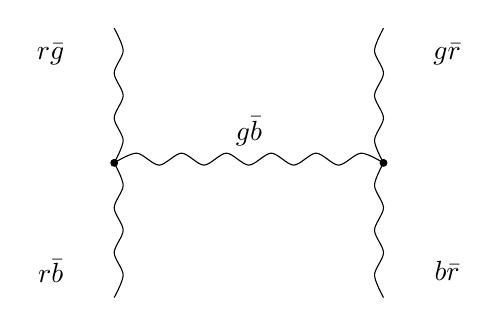
\begin{tikzpicture}[scale=0.95]
\draw[smooth] plot coordinates {
(-1.8,-1.8) (-1.68,-1.50) (-1.80,-1.20) (-1.68,-0.90)
(-1.80,-0.60) (-1.68,-0.30) (-1.8,0)
};
\draw[smooth] plot coordinates {
(-1.8,0) (-1.68,0.30) (-1.80,0.60) (-1.68,0.90)
(-1.80,1.20) (-1.68,1.50) (-1.8,1.8)
};
\draw[smooth] plot coordinates {
(1.8,-1.8) (1.68,-1.50) (1.80,-1.20) (1.68,-0.90)
(1.80,-0.60) (1.68,-0.30) (1.8,0)
};
\draw[smooth] plot coordinates {
(1.8,0) (1.68,0.30) (1.80,0.60) (1.68,0.90)
(1.80,1.20) (1.68,1.50) (1.8,1.8)
};
\draw[smooth] plot coordinates {
(-1.8,0) (-1.50,0.13) (-1.20,-0.03) (-0.90,0.13)
(-0.60,-0.03) (-0.30,0.13) (0,-0.03)
(0.30,0.13) (0.60,-0.03) (0.90,0.13)
(1.20,-0.03) (1.50,0.13) (1.8,0)
};
\node at (-2.65,-1.45) {$r\bar b$};
\node at (-2.65,1.45) {$r\bar g$};
\node at (2.65,-1.45) {$b\bar r$};
\node at (2.65,1.45) {$g\bar r$};
\node at (0,0.42) {$g\bar b$};
\fill (-1.8,0) circle (1.5pt);
\fill (1.8,0) circle (1.5pt);
\end{tikzpicture}
\caption{两个胶子之间交换一个\(g\bar b\)胶子，每条颜色线和反颜色线都连续地穿过顶点。}
\end{figure}

\section{胶子自相互作用与非线性场}

胶子自相互作用改变了QCD的性质。夸克可以通过交换胶子而束缚在一起并形成强子，但胶子也可以通过交换胶子而束缚在一起。因此QCD可以包含完全由胶子自由度构成、不含夸克的复合客体。QED中没有仅由光子构成的相应基本束缚态。

场的语言给出同样的结论。在基本层面上，真空中的两列电磁波彼此穿过。两列胶子波则相互作用并彼此形变。甚至同一个胶子场组态的不同部分之间也能相互施加力。因此胶子场是非线性的。

\begin{classroomqa}
\audiencequestion{图的每一侧都必须出现相同数目的红、绿、蓝标记吗？\lecturetimestamp{01:24:59}}
\lecturerresponse{实用的规则是让每一条颜色线穿过整个图。这种连续性就是颜色守恒。如果一条费米子线在时间中掉头，它的标记就变成相应的反粒子标记或反颜色标记。}
\end{classroomqa}

\begin{classroomqa}
\audiencequestion{图的第一版中所有颜色和反颜色标记都自洽吗？\lecturetimestamp{01:26:00}}
\lecturerresponse{不是。若干标记必须被修正。在自洽的分配中，红线、反蓝线和绿线各自连续地穿过顶点，其中反转的费米子箭头被解释为反粒子。}
\end{classroomqa}

\begin{classroomqa}
\audiencequestion{中间胶子线被当作夸克--反夸克对来处理吗？\lecturetimestamp{01:27:58}}
\lecturerresponse{仅在其颜色记账中如此。胶子并不是字面意义上的夸克--反夸克复合体，但它携带相应的颜色和反颜色性质。}
\end{classroomqa}

在这个阶段，基本规则很简洁：

\begin{itemize}
\item 夸克发射和吸收胶子；
\item 胶子直接与胶子相互作用；
\item 每一条颜色线和反颜色线都必须连续地穿过顶点；
\item 把费米子线在时间中反转，就把它变成相应的反粒子线。
\end{itemize}

\begin{classroomqa}
\audiencequestion{当胶子由所有这些色--反色线表示时，它们仍然是无质量的吗？\lecturetimestamp{01:28:13}}
\lecturerresponse{是的。胶子仍然是无质量的。以下限定涉及强子内部赋予夸克的质量意味着什么。}
\end{classroomqa}

接下来是禁闭和强子结构：为什么从未观察到孤立的色，以及夸克和胶子如何在复合粒子内部组织起来。首先，澄清组分夸克的质量意味着什么是有益的。

\section{探测标度与夸克质量的含义}

想象一个质量为\(m\)的小物体附着在一块柔软、可变形的材料上---一块悬垂的口香糖即可。施加一个非常轻柔的力，慢到柔软材料有时间调整，整个系统一起运动。此时测得的惯性就是小物体的惯性加上附着材料的惯性。

现在以非常高的频率摇动这个小物体。柔软材料没有时间跟随快速运动。它几乎保持静止，而小核心作出响应。此时测得的高频惯性则更接近仅\(m\)的惯性。

\begin{figure}[h]
\centering
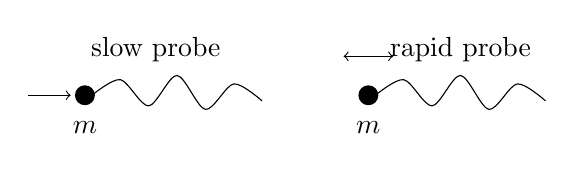
\begin{tikzpicture}[scale=0.9]
\fill (-3,0) circle (4pt);
\node at (-3,-0.45) {$m$};
\draw[smooth] plot coordinates {
(-2.9,0) (-2.5,0.22) (-2.1,-0.15) (-1.7,0.28)
(-1.3,-0.20) (-0.9,0.16) (-0.5,-0.08)
};
\draw[->] (-3.8,0) -- (-3.2,0);
\node at (-2.0,0.65) {slow probe};

\fill (1.0,0) circle (4pt);
\node at (1.0,-0.45) {$m$};
\draw[smooth] plot coordinates {
(1.1,0) (1.5,0.22) (1.9,-0.15) (2.3,0.28)
(2.7,-0.20) (3.1,0.16) (3.5,-0.08)
};
\draw[<->] (0.65,0.55) -- (1.35,0.55);
\node at (2.3,0.65) {rapid probe};
\end{tikzpicture}
\caption{慢速探针使核心及其柔软附着物一起运动，而快速探针最初主要测量核心的响应。}
\end{figure}

这是一个经典类比。推断出的质量取决于所施加力的频率，因为系统不同部分在不同频率下有时间参与响应。

强子内部的夸克被强相互作用的胶子物质以及其他组分所包围。如果能够非常缓慢地拉动一个夸克，整个强子都会响应。此时遇到的惯性将具有核子质量的量级，
\begin{equation}
m_N\sim930\text{--}940\,\mathrm{MeV}.
\end{equation}
如果夸克受到非常剧烈的撞击并在极短时间内被探测，初始响应则与通常赋予轻夸克的更小质量参数相关，大约为
\begin{equation}
m_{u,d}\sim5\text{--}10\,\mathrm{MeV}
\end{equation}
在此处使用的估计中。

因此，``夸克的质量''这一说法需要指明探测的标度。轻柔的低频扰动使延展的复合体运动；剧烈的高频扰动最初只分辨出其中小得多的部分。这个类比并不是重正化的推导，但它说明了为什么用于描述粒子的参数取决于测量它们时所涉及相互作用的频率和波长。这种依赖于标度的参数称为跑动参数或跑动常数。

\begin{classroomqa}
\audiencequestion{这种依赖于频率的质量是否只是对诸如\(\Delta x\,\Delta t\)这样的不确定性关系的重述？\lecturetimestamp{01:33:32}}
\lecturerresponse{不是。这个例子本身已经是一种经典现象。附着在柔软物体上的小质量在快速力作用下以一种方式加速，在缓慢力作用下以另一种方式加速，因为附着材料中有不同数量的部分有时间响应。}
\end{classroomqa}

\begin{classroomqa}
\audiencequestion{前面关于电子电荷的讨论是否涉及同一种标度依赖性？\lecturetimestamp{01:34:04}}
\lecturerresponse{是的。一般的教训是，用于描述粒子的参数取决于探测它们时所涉及相互作用的频率和波长。它们被称为跑动常数。}
\end{classroomqa}

\begin{classroomqa}
\audiencequestion{同样的限定是否适用于赋予夸克的分数电荷？\lecturetimestamp{01:34:36}}
\lecturerresponse{适用。必须仔细定义夸克电荷意味着什么。在这个层面上，它是相对于质子电荷引用的；更完整的定义是另一个单独的讨论。}
\end{classroomqa}

\editorialnote{固定的分数电荷量子数与依赖于标度的相互作用耦合是不同的。耦合的跑动不会改变\(+\tfrac23\)或\(-\tfrac13\)味标签本身。}

\begin{classroomqa}
\audiencequestion{为什么色的记账总是使用一个夸克和一个反夸克？为什么两个夸克不能形成相应的对象？\lecturetimestamp{01:34:55}}
\lecturerresponse{这是一个重要的问题，但它的答案属于下一次关于允许的色组合和禁闭的讨论。}
\end{classroomqa}

\begin{classroomqa}
\audiencequestion{如果单个夸克无法被孤立出来，那么分数电荷、色以及夸克模型又是如何被推断出来的？\lecturetimestamp{01:35:17}}
\lecturerresponse{这一图景是从许多线索连同明显的矛盾中逐渐浮现出来的。强子谱模式暗示了夸克组分；Delta态暴露出与费米统计的冲突；而夸克的永久禁闭又提供了另一个奇特的事实。夸克提议出现于1960年代初，南部阳一郎提出了色思想的一个重要早期版本，许多物理学家在随后的大约十年间拼合并检验了完整的结构。它不是某一次观测或某一个人的结果。}
\end{classroomqa}

\begin{classroomqa}
\audiencequestion{为什么只有八种胶子，而不是九种表观的色--反色组合？\lecturetimestamp{01:37:24}}
\lecturerresponse{关于为什么对角和不是额外的一种胶子的详细解释被推迟了。}
\end{classroomqa}

\begin{classroomqa}
\audiencequestion{这段关于QCD的讨论忽略了电子吗？\lecturetimestamp{01:37:33}}
\lecturerresponse{是的。QCD正以讨论QED时可以暂时忽略夸克的同样方式被孤立出来。这些分离的部门最终必须被组合进一个包含夸克、电子、光子以及其他粒子的更大结构之中。那一更大综合的某些部分已经完成，某些部分仍不完整。物理学常常通过孤立一个子系统、理解它、然后再把各个部分重新拼合起来而推进。}
\end{classroomqa}
